\documentclass{article}
\usepackage{graphicx}
\usepackage[utf8]{inputenc}
\usepackage[T1]{fontenc}
\usepackage{pgfplots}
\usepackage{pgfplotstable} 
\usepackage{titlesec}
\usepackage{lipsum}
\usepackage{authblk}
\usepackage{algorithm}
\usepackage{amsmath}
\usepackage[noend]{algpseudocode}
\usepackage {tikz}
\usetikzlibrary {positioning}

\titleformat{\chapter}[display]{\normalfont\bfseries}{}{0pt}{\Large}

\begin{document}

\title{Projeto e Análise de Algoritmos: Trabalho Prático 1}
\author{João Mateus de Freitas Veneroso}
\affil{Departamento de Ciência da Computação da Universidade Federal de Minas Gerais}

\maketitle

\section{Introdução}

Este relatório descreve a implementação do trabalho prático 2 da disciplina Projeto e Análise de Algoritmos. 
O trabalho consistiu em resolver um problema de compartilhamento de viagens por meio de três paradigmas diferentes:
força bruta, programação dinâmica e algoritmos gulosos.

\section{Força Bruta}

O algoritmo de força bruta descrito abaixo é o mesmo implementado no Trabalho Prático 1.

O algoritmo \ref{alg:alg_1} implementa uma solução de força bruta para o problema de compartilhamento de viagens. 
Primeiro inicializa-se o benefício máximo $ b^* $ com um valor negativo, dessa
forma qualquer configuração válida vai proporcionar um benefício maior. A partir daí, no loop das linhas 5-10, para cada configuração
válida, calcula-se o benefício total e atualiza-se o valor de $ b^* $ se este benefício for maior do que qualquer um encontrado até então.
Além disso, a variável $ G_p^* $ guarda a configuração que proporcionou o maior benefício. Ao final do algoritmo, $ b^* $ guarda o valor 
do benefício máximo para o grafo $ G $ e $ G_p^* $ guarda a configuração que proporcionou este benefício. 

A complexidade deste algoritmo depende do número de configurações $ G_p $ diferentes e do custo da função $ ConstraintsAreValid $. O número de 
configurações $ G_p $ diferentes é $ 2^m $ para $ m $ igual ao número de arestas no grafo $ G $. Pois, cada aresta pode estar presente ou
não em $ G_p $ e nós queremos as combinações possíveis para todas as arestas m. O custo da função $ ConstraintsAreValid $ depende do número de 
arestas, pois, para cada aresta $ (u,v) $, temos de verificar se ela é a única aresta que sai do vértice $ u $, se o vértice $ v $ é um motorista
e se $ v $ possui espaço para acomodar todos os passageiros de $ u $. Como todas estas operações tem custo constante, a função $ ConstraintsAreValid $ 
tem custo $ O(m) $. Por último, a linha 7 calcula a soma dos pesos de todas as arestas também com custo $ O(m) $. Logo, 
a complexidade total do algoritmo é $ 2m2^m $ e o algoritmo é $ O(m2^m) $.

\begin{algorithm}
\caption{MaximizeBenefit}
\begin{algorithmic}[1]
\Procedure{MaximizeBenefit}{G(V,A)}

\State $ b^* \gets -1 $
\State $ G_p^* \gets \emptyset $
\item \ForAll{\textit{$ G_p = (V, A_p) : A_p \subseteq G.A $}}

\If {\textit{ConstraintsAreValid($G_p$)}}
  \State $ \textit{b} \gets \sum_{(v_i, v_j) \in A_p} B(v_i, v_j) $
  \If {$ b > b^* $}
    \State $ b^* \gets b $
    \State $ G_p^* \gets G_p $
  \EndIf
\EndIf
\EndFor
\EndProcedure
\end{algorithmic}
\label{alg:alg_1}
\end{algorithm}

Uma melhora ainda pode ser alcançada se deixarmos de testar parte das configurações inválidas de $ G $. Sabemos que 
um passageiro somente pode pegar carona em um carro, portanto, qualquer combinação $ G_p $ onde existirem arestas $ (u, v_i), (u, v_j) : i \neq j $
é inválida. Dessa forma, basta manter uma única aresta ativa por vez na lista de adjacência de cada vértice. É necessário lembrar 
que um vértice pode representar um motorista sem passageiros ou um grupo de passageiros que não vai pegar carona com ninguém, 
portanto, o número total de combinações se torna $ \sum_{v \in V} G.Adj(v) + 2 $ e, no pior caso (um grafo completo), 
o número de combinações se torna $ O(n^n) $ onde n é o número de vértices no grafo $ G $. 
Feitas estas considerações, a complexidade assintótica do algoritmo é $ O(mn^n) $. Apesar da complexidade parecer 
pior do que o algoritmo descrito anteriormente, devido a forma como o algoritmo é construído ele é sempre necessariamente
melhor ou igual ao algoritmo anterior. Pois, no máximo, ele testa todas as combinações de arestas $ 2^m $.
O algoritmo de força bruta implementado em Python para este trabalho utiliza este método.

A complexidade de espaço do algoritmo original e da versão aprimorada é $ O(n + m) $, pois o grafo é armazenado na forma de listas de adjacência.

\section{Programação Dinâmica}

Em qualquer solução válida para o problema dos compartilhamentos de viagem, os passageiros-motoristas tem de decidir se vão
atuar exclusivamente como passageiros ou motoristas devido às restrições do problema. Dessa forma, sendo k o número de passageiros-motoristas, 
ao variar quais deles atuam como passageiros e quais atuam como motoristas, existem $ 2^k $ combinações possíveis que dão origem a problemas distintos. 
Cada um destes problemas pode ser pensado como um grafo bipartido G(V,A) onde os vértices de passageiros pertencem a um subconjunto de V e os vértices 
de motoristas pertencem a um outro subconjunto de V, sendo que todas as arestas conectam um vértice passageiro a um vértice motorista e os dois subconjuntos
são disjuntos.

\begin{figure}
  \center
  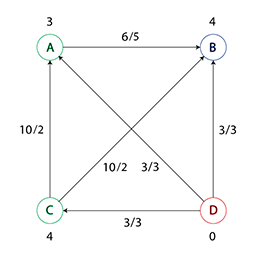
\includegraphics[width=128px]{graph.png}
  \caption{Exemplo do problema de compartilhamento de viagens modelado em forma de grafo}
  \label{fig:graph}
\end{figure}

\begin{figure}
  \center
  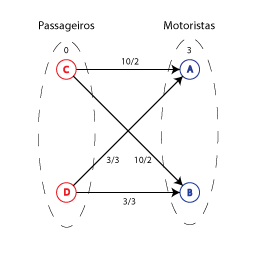
\includegraphics[width=164px]{bipartite_graph.png}
  \caption{Grafo bipartido após definição dos passageiros e motoristas no grafo da figura \ref{fig:graph}}
  \label{fig:bipartite_graph}
\end{figure}

A figura \ref{fig:graph} mostra um exemplo do probema de compartilhamento de viagens modelado na forma de um grafo, onde vértices
vermelhos representam grupos de passageiros, vértices azuis representam motoristas e vértices verdes representam passageiros-motoristas. Os números
próximos aos vértices representam a capacidade do veículo e os números próximos às arestas $ (v_i, v_j) $ representam o 
benefício do compartilhamento $ B(v_i, v_j) $ e o número de passageiros na viagem $ Q(v_i, v_j) $ separados por uma barra.
Perceba que os vértices A e C são passageiros-motoristas e os demais vértices são passageiros ou motoristas exclusivos. Ao selecionar 
o vértice A como motorista e o vértice C como passageiro, podemos modelar o problema com o grafo bipartido da figura \ref{fig:bipartite_graph}.
Para cada uma das combinações de passageiros e motoristas podemos construir um grafo bipartido similar. Nesta forma, o problema passa a se parecer
bastante com o \textit{0-1 Multiple Knapsack Problem}, com a diferença que alguns items podem estar restritos à sacolas específicas. 
No caso, as sacolas representam os carros e os itens representam os grupos de passageiros.
Além disso, é possível mapear o \textit{0-1 Multiple Knapsack Problem} no problema de compartilhamento de viagens se considerarmos 
o caso em que todos os passageiros podem pegar carona em todos os veículos. Logo, o problema do compartilhamento de viagens é NP-difícil.

Dado um grafo $ G(V,A)$, cada motorista $ v_j $ dá origem a um \textit{0-1 Knapsack Problem}. Pois, cada aresta $ (v_i, v_j) \in G.A $
representa uma possbilidade do grupo de passageiros $ v_i $ seguir viagem com $ v_j $. Logo, para maximizar o benefício dos
compartilhamentos do motorista $ v_j $ ($ B_{max}(G, v_j) $) é preciso escolher o conjunto de arestas $ (v_i, v_j) $ que confira o maior benefício
sem exceder a capacidade do carro, que é basicamente a definição do \textit{0-1 Knapsack Problem}. No entanto, a forma como 
um motorista maximiza o benefício dos seus compartilhamentos influencia como os outros motoristas podem
maximizar os seus compartilhamentos. Logo, assumindo que o motorista $ v_j $ está levando o grupo de passageiros $ X $, o próximo
motorista deverá maximizar seu benefício com base no grafo $ G'(V - X - v_j, A') $, sendo que $ A' $ é o conjunto de arestas original 
$ A $ sem as arestas que contém $ v_j $ ou qualquer um dos passageiros levados por ele. No caso de motoristas que podem ser passageiros,
também existe a possibilidade do motorista $ v_j $ não levar passageiro nenhum. Nesse caso, as arestas incidentes em $ v_j $
serão apagadas do grafo $ G $, mas as arestas que saem de $ v_j $ serão mantidas e, o vértice $ v_j $ também será mantido.

Se o motorista $ v_j $ decide levar um passageiro $ v_i $, os demais motoristas vão maximizar seus benefícios sem considerar o 
passageiro $ v_i $ no grafo. Por conta disso, o benefício encontrado não será necessariamente máximo. Por exemplo, tome o caso em que
$ v_j $ pode levar um dos grupos de passageiros $ \{ p_1 = 12/2, p_2 = 20/1, p3 = 1/1 \} $ onde o primeiro valor associado a cada grupo representa o seu benefício
e o segundo valor representa o número de pessoas naquele grupo (note que a barra não representa divisão nesse caso).
Assumindo que $ v_j.capacidade = 2 $, $ v_j $ maximiza o benefício dos seus compartilhamentos se escolher os passageiros $ \{ p_2, p_3 \} $ auferindo um
benefício total de $ 21 $. Agora assuma que existe um outro motorista $ v_{j+1} $ que pode compartilhar viagem apenas com $ p_2 $. Nesse caso,
o motorista $ v_{j+1} $ ficará impedido de compartilhar essa viagem. No entanto, o benefício máximo dos compartilhamentos seria claramente 
maior se $ v_j $ tivesse escolhido levar $ \{ p_1 \} $ ao invés de $ \{ p_2, p_3 \} $. 

Por conta da incapacidade de prever localmente qual é o benefício total máximo do plano de compartilhamento, é necessário testar 
qual o benefício máximo para cada combinação de vértices no grafo $ G $. Considere os motoristas $ \{ D_1, D_2, ..., D_n \} $.
Agora, assuma uma combinação de passageiros válida em $ D_i $ que faz parte de um plano de benefício máximo $ B_{max}(G, D_i) $ 
e remova de G todos os passageiros escolhidos por $ D_i $ e o próprio motorista $ D_i $, gerando o grafo $ G' $. Ora,
$ B_{max}(G, D_{i}) = B(D_i) + B_{max}(G', D_{i - 1}) $, onde $ B(D_i) $ é a soma dos benefícios dos passageiros de $ D_i $.
Ou seja, o problema tem subestrutura ótima. A prova deste teorema é que, se $ B(G, D_{i}) $ é ótimo mas a configuração que gera
o benefício $ B(G', D_{i - 1}) $ não é máxima, poderíamos substituí-la por uma configuraçãp que gerasse um benefício total
maior, no entanto, isso contradiz a hipótese inicial que $ B_{max}(G, D_{i}) $ era máximo. Então, $ B_{max}(G, D_{i}) $ tem de ser
máximo.

Todavia, nós não sabemos qual é a configuração de passageiros de benefício máximo para $ D_i $. Portanto, devemos testar
todas as possibilidades e escolher aquela que oferece o maior benefício. Finalmente, podemos construir a seguinte equação 
de recorrência:

\begin{equation}
  B_{max}(G, D_i) = 
  \begin{cases}
    0, & \textit{se $ G = \emptyset $}.\\
    \max\limits_{P_{comb} \subseteq D_i.P} B_{max}(G', D_{i-1}) + \sum\limits_{p \in P_{comb}} B(p), & \textit{caso contrário}.\\
  \end{cases}
\end{equation}

onde $ P_{comb} $ representa uma das combinações de passageiros do motorista $ D_i $, e $ D.P $ são todos os potencias passageiros do
motorista $ D_i $ no grafo $ G $. $ G' $ depende da escolha dos passageiros como explicado nos parágrafos anteriores e $ B(P) $ é o benefício do passageiro P.
A ordem de escolha dos motoristas $ D_i $ não é importante uma vez que todas as possíveis combinações de
passageiros acabam sendo testadas de uma forma ou de outra. 

A implementação ingênua desta equação de recorrência acaba calculando várias vezes o mesmo problema, pois, o poblema $ B(G, D_i) $ 
pode ocorrer mais de uma vez na árvore de recursão. Portanto, podemos ganhar eficiência ao
salvar os resultados dos cálculos em uma tabela.

% O \textit{0-1 Knapsack Problem} pode ser resolvido de forma simples gerando uma tabela onde as linhas representam os passageiros
% $ \{ p_1, p_2, ..., p_n\} \in D_j.P $ e as colunas representam a capacidade de $ D_j $ de 1 até $ D_j.capacidade $. Então, calculamos
% para cada linha, o benefício máximo dado o limite imposto pelas colunas. Na próxima linha, verificamos se podemos incluir o próximo passageiro 
% para cada uma das capacidades e, se isso não for possível, repetimos o valor da célula de cima. Se for possível incluir o passageiro, então
% verificamos o valor da linha de cima com a capacidade da coluna atual menos o número de passageiros adicionados. Devido a uma limitação
% de espaço este algoritmo não será explicado em mais detalhes. No entanto, o código implementa ele conforme os passos aqui descritos.

No caso do cálculo do benefício máximo, podemos aplicar uma abordagem de programação dinâmica \textit{Bottom Up}.
Digamos que $ D = {D_1, D_2, ..., D_n} $ é a lista dos motoristas no grafo $ G $. E, o grafo G possui $ 2^n $ 
subgrafos com combinações diferentes dos vértices $ G.V $. Consideremos agora o problema de encontrar 
o benefício máximo para cada uma das combinações de $ G.V $ considerando apenas os motoristas $ \{ D_1, D_2, ..., D_i \} $.
Como demonstrado anteriormente, este problema tem subestrutura ótima e as construções para $ D_{i+1}, D_{i+2}, ... $
dependem de sua solução. Podemos produzir uma matriz $ B_{max} $ com $ n $ linhas representando os conjuntos
de motoristas e $ 2^n $ colunas representando todas as possíveis combinações $ V_j \subseteq G.V $, sendo que os índices 
são a codificação binária das combinações. Por exemplo, $ \{ 0 \Rightarrow \emptyset, 1 \Rightarrow \{ V_1\},
2 \Rightarrow \{ V_2\}, 3 \Rightarrow \{ V_1, V_2\}, ... \} $. Cada célula $ B_{max}[i][j] $ representa o benefício máximo
considerando apenas os motoristas $ \{ D_1, D_2, ..., D_i \} $ no grafo $ G' $ onde $ v_k \in V_j \forall v_k \in G'.V $.
O tamanho total da matriz $ B_{max} $ será $ O(n2^n) $ sendo $ n $ o número de vértices do grafo $ G $.

\begin{algorithm}
\caption{DPMaximizeBenefit}
\begin{algorithmic}[1]
\Procedure{DPMaximizeBenefit}{G(V,E)}

\State $ Drivers := GetDrivers(G) $
\State $ B_{max} := Array[Drivers.length] $
\State $ Combinations := |G.V|^2 $
\State $ i := 0 $
\item \ForAll{$ i < Drivers.length $}
  \State $ B_{max}[i] := Array[Combinations] $
\EndFor

\item \ForAll{$ D_i \in Drivers $}
  \ForAll{$ V_j \subseteq G.V $}
    \If {$ D_i \in V_j $}
      \State $ MaxBenefit := 0 $
      \If {$ i > 0 $}
      \State $ MaxBenefit := B_{max}[i-1][j] $
      \Comment Benefit without adding any passengers.
      \EndIf

      \State Remove $ D_i $ from $ G.V $
      \ForAll{$ P_{comb} \subseteq D_i.P $}
        \State $ Benefit := 0 $
        \ForAll{$ p \in P_{comb} $}
          \State $ Benefit := Benefit + B(p) $
          \State Remove $ p $ from $ G.V $
        \EndFor
       
        \State $ CombIndex := GetCombIndex(G.V) $
        \State $ Benefit := Benefit + B_{max}[i - 1][CombIndex] $
        \If {$ Benefit > MaxBenefit $}
          \State $ MaxBenefit := Benefit $
        \EndIf

        \State Add $ D_i $ back to $ G.V $
        \ForAll{$ p \in P_{comb} $}
          \State $ Benefit := Benefit + B(p) $
          \State Add $ p $ back to $ G.V $
        \EndFor
      \EndFor
    \Else
      \State $ B_{max}[i][j] = 0 $  
      \If {$ i > 0 $}
        \State $ B_{max}[i][j] = B_{max}[i-1][j] $  
      \EndIf
    \EndIf
  \EndFor
\EndFor

\State $ MaxBenefit := 0 $
\State $ i := Drivers.length - 1 $
\item \ForAll{$ V_j \subseteq G.V $}
  \If {$ B_{max}[i][j] > MaxBenefit $}
    \State $ MaxBenefit := B_{max}[i][j] $
  \EndIf
\EndFor

\Return $ MaxBenefit $
\EndProcedure
\end{algorithmic}
\label{alg:dynamic_programming}
\end{algorithm}

Finalmente, o algoritmo para a abordagem \textit{Bottom Up} está descrito em \ref{dynamic_programming}. Os
nomes de todas as variáveis são equivalentes aos definidos nos últimos parágrafos. A única informação nova é a 
função \textit{GetCombIndex(G.V)} que retorna o índice $ j $ na tabela $ B_{max} $ para o subconjunto de vértices do grafo $ G $.
Para $ n $ igual ao número de vértices no grafo $ G $, o loop principal é chamado no máximo $ n $ vezes. O loop secundário é chamado 
exatamente $ 2^n $ vezes e o terceiro loop é chamado no máximo $ 2^n $ vezes. Por último, o loop final é chamado exatamente $ 2^n $
vezes. Portanto, a complexidade do algoritmo é $ n2^n2^n + 2^n = n2^{2n} + 2^n $ e o algoritmo é $ O(n4^n) $. A complexidade de espaço
do algoritmo é $ O(n2^n) $ como exposto anteriormente, mas podemos reduzí-la para $ O(2^n) $ se salvarmos apenas a linha anterior
em cada iteração e, na iteração final, podemos simplesmente escolher a combinação que dê o benefício máximo sem salvar
as respostas para cada combinação. Não é uma solução muito eficiente, mas já é bem melhor do que o algoritmo de força bruta. Devido 
ao fato do problema do compartilhamento de viagens ser NP-difícil, todas as soluções serão de ordem exponencial se $ P \neq NP $.

\section{Algoritmo Guloso}

O algoritmo guloso para o problema do compartilhamento de viagens o problema de escolher o subconjunto ótimo de passageiros para
cada motorista a cada iteração como uma instância separada do \textit{0-1 Knapsack Problem}. Basicamente, os itens da sacola (passageiros) 
serão ordenados por ordem não crescente de eficiência, sendo que a eficiência é definida por:

\[ 
\frac{\textit{benefício}}{\textit{número de passageiros na viagem}}
\]

A estratégia gulosa vai escolher os itens nesta ordem até que o carro não comporte mais nenhum passageiro. Adicionalmente,
conferimos se colocar apenas o passageiro de maior benefício dentro do carro vai conferir um benefício maior do que a estratégia
descrita e, se este for o caso, substituímos os passageiros escolhidos pelo passageiro de maior benefício. Essa estratégia não
garante uma solução ótima para o problema, mas é bastante rápida e tem complexidade $ O(nlogn) $ devido à ordenação dos passageiros.

Dado um grafo $ G $, escolheremos o motorista cujo benefício calculado pelo \textit{0-1 Knapsack Problem} é o maior entre
todos os motoristas do grafo. Então, adicionamos o benefício obtido ao benefício total e retiramos as arestas 
que saem dos passageiros e do motorista do grafo $ G $, produzindo o grafo $ G' $. Repetimos o processo até que não haja mais 
motoristas no grafo e, ao final do processo, obtemos o benefício total. Da mesma forma que o \textit{0-1 Knapsack Problem}, esta estratégia não
produz necessariamente um resultado ótimo. No entanto, a complexidade para a escolha do motorista é $ n^2logn $ e este processo é repetido
no máximo $ n $ vezes, portanto, a complexidade do algoritmo é $ O(n^3logn) $, que é polinomial e, portanto, consideravelmente melhor do 
que as alternativas exatas.

\begin{algorithm}
\caption{GreedyMaximizeBenefit}
\begin{algorithmic}[1]
\Procedure{GreedyMaximizeBenefit}{G(V,E)}

\State $ Plan := \emptyset $
\State $ MaxBenefit := 0 $
\item \While{$ G.E \neq \emptyset $}
  \State $ BestDriver := null $
  \State $ BestPlan := \emptyset $
  \State $ MaxDriverBenefit := 0 $
  \item \ForAll{$ D_i \in G.Drivers $}
    \State $ S := KnapsackGreedy(D_i, G.V) $
    \State $ DriverBenefit := \textit{GetBenefit(S)} $
    \If {$ DriverBenefit > MaxDriverBenefit $}
      \State $ MaxDriverBenefit = DriverBenefit $
      \State $ BestDriver = D_i $
      \State $ BestPlan = S $
    \EndIf
  \EndFor

  \State Update Plan with the edges in BestPlan
  \State Remove edges from best driver and all passengers in graph G
  \State $ MaxBenefit = MaxBenefit + MaxDriverBenefit $
\EndWhile

\Return MaxBenefit

\EndProcedure
\end{algorithmic}
\label{alg:greedy_algorithm}
\end{algorithm}

A abordagem gulosa para o problema da maximização de benefício no grafo de compartilhamento de viagens está
descrita no algoritmo \ref{alg:greedy_algorithm}. A função \textit{KnapsackGreedy} utiliza a estratégia gulosa descrita anteriormente
para selecionar o melhor conjunto de passageiros para o motorista $ D_i $. A função \textit{GetBenefit} simplesmente
calcula o benefício total do conjunto de passageiros selecionados pelo \textit{KnapsackGreedy}.

\section{Experimentos}

\begin{figure}
  \center
  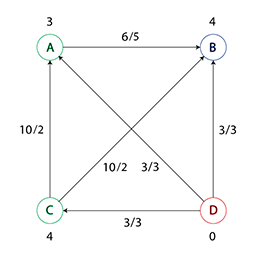
\includegraphics[width=128px]{graph.png}
  \caption{Número de vértices X Tempo de execução}
  \label{fig:execution_time}
\end{figure}

\begin{table}
\centering
\begin{tabular}{ |l|l|l|l| }
  \hline
  Vértices & Algoritmo Guloso & Algoritmo Exato & Aproximação \\
  \hline
  1  & 65               & 233106 & 233106\% \\
  2  & 33               & 220774 & 220774\% \\
  3  & 22               & 220127 & 220127\% \\               
  4  & 15               & 278959 & 278959\% \\               
  5  & 13               & 211959 & 211959\% \\              
  6  & 7                & 223152 & 223152\% \\               
  7  & 4                & 247336 & 247336\% \\               
  8  & 2                & 285716 & 285716\% \\               
  9  & 2                & 235183 & 235183\% \\
  10 & 2                & 302967 & 302967\% \\               
  11 & 2                & 302967 & 302967\% \\               
  12 & 2                & 302967 & 302967\% \\               
  13 & 2                & 302967 & 302967\% \\               
  14 & 2                & 302967 & 302967\% \\               
  15 & 2                & 302967 & 302967\% \\               
  16 & 2                & 302967 & 302967\% \\               
  17 & 2                & 302967 & 302967\% \\               
  18 & 2                & 302967 & 302967\% \\               
  19 & 2                & 302967 & 302967\% \\               
  20 & 2                & 302967 & 302967\% \\               
  \hline
\end{tabular}
\caption{Aproximação pelo algoritmo guloso}
\label{tab:greedy_approximation}
\end{table}

Foram feitos experimentos com grafos completos variando entre 1 e 20 vértices em cada uma dos três paradigmas implementados. A figura
\ref{fig:execution_time} descreve o desempenho de cada um dos algoritmos propostos. No caso do algoritmo guloso também foi 
calculado quanto a solução gulosa se aproximou da solução ótima. O resultado está descrito na tabela \ref{tab:greedy_approximation}.

\section{Conclusão}

Este relatório descreveu a implementação do trabalho prático 2 da disciplina Projeto e Análise de Algoritmos. Entre as três abordagens
propostas, a abordagem gulosa apresentou claramente o melhor desempenho chegando a uma aproximação média de 90\% da resposta ótima
em um tempo 100 vezes menor do que as abordagens exatas. A programação dinâmica não mostrou um ganho muito grande em relação à força
bruta devido ao \textit{overhead} na montagem da tabela de respostas. No entanto, talvez o resultado seja diferente para grafos 
significativamente maiores.

\end{document}
